\documentclass[a4paper]{article}
\usepackage{vntex}
\usepackage[colorlinks]{hyperref}
%\usepackage[english,vietnam]{babel}
%\usepackage[utf8]{inputenc}

%\usepackage[utf8]{inputenc}
%\usepackage[francais]{babel}
\usepackage{a4wide,amssymb,epsfig,latexsym,multicol,array,hhline,fancyhdr}

\usepackage{amsmath}
\usepackage{lastpage}
\usepackage[lined,boxed,commentsnumbered]{algorithm2e}
\usepackage{enumerate}
\usepackage{color}
\usepackage{graphicx}							% Standard graphics package
\usepackage{array}
\usepackage{tabularx, caption}
\usepackage{multirow}
\usepackage{multicol}
\usepackage{rotating}
\usepackage{graphics}
\usepackage[left = 2.5cm, right = 2cm]{geometry}
\usepackage{setspace}
\usepackage{epsfig}
\usepackage{tikz}
\usepackage{hyperref}
\usepackage{mdframed}
\usepackage{lipsum}
\hypersetup{urlcolor=blue,linkcolor=black,citecolor=black,colorlinks=true} 
%\usepackage{pstcol} 								% PSTricks with the standard color package

\newtheorem{theorem}{{\bf Định lý}}
\newtheorem{property}{{\bf Tính chất}}
\newtheorem{proposition}{{\bf Mệnh đề}}
\newtheorem{corollary}[proposition]{{\bf Hệ quả}}
\newtheorem{lemma}[proposition]{{\bf Bổ đề}}


%\usepackage{fancyhdr}
\setlength{\headheight}{40pt}
\pagestyle{fancy}
\fancyhead{} % clear all header fields
\fancyhead[L]{
 \begin{tabular}{rl}
    \begin{picture}(25,15)(0,0)
    \put(0,-8){
\includegraphics[width=8mm, height=8mm]{hcmut.png}}
    %\put(0,-8){\epsfig{width=10mm,figure=hcmut.eps}}
   \end{picture}&
	%
\includegraphics[width=8mm, height=8mm]{hcmut.png} & %
	\begin{tabular}{l}
		\textbf{\bf \ttfamily Trường Đại Học Bách Khoa Tp.Hồ Chí Minh}\\
		\textbf{\bf \ttfamily Khoa Khoa Học và Kỹ Thuật Máy Tính}
	\end{tabular} 	
 \end{tabular}
}
\fancyhead[R]{
	\begin{tabular}{l}
		\tiny \bf \\
		\tiny \bf 
	\end{tabular}  }
\fancyfoot{} % clear all footer fields
\fancyfoot[L]{\scriptsize \ttfamily Operating System 2018 - 2019}
\fancyfoot[R]{\scriptsize \ttfamily Trang {\thepage}/\pageref{LastPage}}
\renewcommand{\headrulewidth}{0.3pt}
\renewcommand{\footrulewidth}{0.3pt}


%%%
\setcounter{secnumdepth}{4}
\setcounter{tocdepth}{3}
\makeatletter
\newcounter {subsubsubsection}[subsubsection]
\renewcommand\thesubsubsubsection{\thesubsubsection .\@alph\c@subsubsubsection}
\newcommand\subsubsubsection{\@startsection{subsubsubsection}{4}{\z@}%
                                     {-3.25ex\@plus -1ex \@minus -.2ex}%
                                     {1.5ex \@plus .2ex}%
                                     {\normalfont\normalsize\bfseries}}
\newcommand*\l@subsubsubsection{\@dottedtocline{3}{10.0em}{4.1em}}
\newcommand*{\subsubsubsectionmark}[1]{}
\makeatother
\begin{document}

\begin{titlepage}
\begin{center}
\large ĐẠI HỌC QUỐC GIA THÀNH PHỐ HỒ CHÍ MINH \\
TRƯỜNG ĐẠI HỌC BÁCH KHOA \\
KHOA KHOA HỌC - KỸ THUẬT MÁY TÍNH 
\end{center}

\vspace{1cm}

\begin{figure}[h!]
\begin{center}

\includegraphics[width=3cm]{hcmut.png}
\end{center}
\end{figure}

\vspace{1cm}

\begin{center}
\begin{tabular}{c}
\Large  \textbf{{\Large Course: OPERATING SYSTEM}}\\
~~\\
\hline
\hline
\\
\vspace{0.5cm}
\Large \textbf{{\Huge Assignment \#1 - System Call  }}\\
\Large \textbf{{\Huge Report  }}\\
\\
\hline
\hline
\end{tabular}\\
\vspace{0.5cm}
\Large  \textbf{GVHD:} \Large \textbf{Huỳnh Nam}\\
\end{center}

\vspace{2.8cm}


\begin{table}[h]

\begin{tabular}{rrl}


\end{tabular}
\end{table}

\vspace{2.5cm}

\begin{center}
{\large TP. HỒ CHÍ MINH, THÁNG 4/2019}
\end{center}
\end{titlepage}


%\thispagestyle{empty}
\newpage
\textbf{\Large Danh sách thành viên}
\begin{enumerate}{}  
\item \large Nguyễn Tiến Phát - 1712572
\item \large  Nguyễn Lục Sâm Bảo - 1710598
\end{enumerate}
\\
\newpage \tableofcontents
%\newpage \listoffigures
% \newpage \listoftables

\newpage

%%%%%%%%%%%%%%%%%%%%%%%%%%%%%%%%%
\section{Adding new system calls}
\textbf{SYSTEM CALL - procsched:}
\begin{itemize}
\item Tại địa chỉ thư mục\textbf{ arch/x86/entry/syscalls/}, các system calls được liệt kê trong các file \textbf{.tbl}.\\
Để thông báo về system calls mới, mở file\textbf{ syscall\_32.tbl}, thêm dòng sau vào cuối file: [number] i386 procsched sys\_procsched.\\
Tương tự với file \textbf{syscall\_64.tbl}: [number] x32 procsched sys\_procsched.\\
\textbf{QUESTION:} Ý nghĩa của \textbf{i386}, \textbf{procsched} và \textbf{sys\_procsched} ?\\
\textbf{ANSWER:}
\begin{itemize}
    \item \textbf{i386} là ABI, hay còn gọi là giao diện nhị phân ứng dụng, là hai giao diện giữa hai module chương trình nhị phân.\href{https://en.wikipedia.org/wiki/Application_binary_interface}{Reference}
    \item \textbf{procsched} đơn giản là tên của system call, cụ thể ở đây là procshed.
    \item \textbf{sys\_procsched} là entry point. Entry point là tên của một hàm gọi đến để xử lý một syscall.Quy ước đặt tên của entry point là tên syscall với tiền tố là sys\_.
\end{itemize}
\item Mở file the đường dẫn include/linux/syscalls.h và thêm dòng sau:
     \\
{{\color{blue} struct} proc\_segs;}\\
\tab{asmlinkage {\color{blue} long} sys\_procsched( {\color{blue} int} pid, {\color{blue} struct} proc\_segs* info);}\\
\textbf{QUESTION:} Ý nghĩa của 2 dòng trên ?\\
\textbf{ANSWER:}
\begin{itemize}
    \item Hai dòng trên thông báo cho hệ thống xác nhận định nghĩa của {\color{blue} struct} \textbf{proc\_segs} và hàm \textbf{sys\_procsched()}.
    \item \textbf{asmlinkage} là một \#define cho trình dịch gcc với ý thông báo rằng tham số sẽ được lấy trực tiếp trên stack chứ không phải từ thanh ghi.
\end{itemize}
\item Tại địa chỉ arch/x86/kernel, tạo 1 file source \textbf{sys\_procsched.c} và hiện thực code theo hướng dẫn, hoàn chỉnh source code tại {\color{blue} //TODO}. Sau khi hiện thực xong ,dùng \textbf{Vim editor} để chỉnh sửa  Makefile, bằng cách thêm dòng : \textbf{obj-y += sys\_procsched.o} ở cuối file Makefile để build \textbf{sys\_procsched}.
\end{itemize}
 \newpage
\section{System calls Implementation}
\textbf{Các bước thực hiện:}
\begin{itemize}
    \item Để tiến hành, chúng ta cần chuẩn bị một máy ảo để cài đặt \textbf{Ubuntu OS}. Ở đây chúng tôi dùng máy ảo \textbf{Oracle VM VirtualBox} để cài đặt \textbf{Ubuntu version 12.04}
    \item Tiếp theo tiến hành cài đặt package bằng một số câu lệnh:\\
   \fbox{
   \parbox{0.8\linewidth}{
		\$ sudo apt-get update\\
		\$ sudo apt-get install build-essential\\
		\$ sudo apt-get install kernel-package
	    }
        }

\textbf{QUESTION:} Tại sao chúng ta cần cài đặt kernel-package?\\
\textbf{ANSWER:}
    \begin{itemize}
        \item \textbf{kernel-package} là một package được phát triển bên ngoài mong muốn dúng để tự động hóa một số bước thường xuyên trong việc yêu cầu biên dịch và cài đặt một customer kernel.
        \item Nếu không có thì chúng ta không thể đụng vào cái file hệ thống khi cài đặt kernel.
    \end{itemize}
\item Tiếp theo chúng ta tạo thư mục \textbf{kernelbuild} ở thư mục \textbf{Home}. Sau đó thực hiện download kernel source và giải nén trong thư mục \textbf{kernelbuild}. Chúng ta chọn bản \textbf{4.4.56}, thực hiện qua 2 command line sau:\\
     \fbox{
   \parbox{0.8\linewidth}{
        \$ mkdir \~/kernelbuild\\
		\$ wget https://cdn.kernel.org/pub/linux/kernel/v4.x/linux-4.4.56.tar.xz\\
		\$  tar -xvJf linux-4.4.56.tar.xz
	    }
        }\\
\textbf{QUESTION:} Tại sao chúng ta phải sử dụng một source kernel khác mà không sử dụng trực tiếp kernel gốc(kernel đang chạy trên OS)?\\
\textbf{ANSWER:}
    \begin{itemize}
        \item Để giảm bớt độ rủi ro khi build trực tiếp trên OS. Vẫn có thể build trực tiếp được nhưng tỉ lệ xảy ra lỗi rất cao, khó fix bug.
    \end{itemize}

\item Sau khi thực hiện cấu hình thành công customer kernel, chúng ta tiến hành hiện thực system call:
    \begin{itemize}
        \item Đặc tả {\color{blue}struct} proc\_segs với các biến bao gồm:\\
        \fbox{
        \parbox{0.8\linewidth}{
            {\color{blue}struct} proc\_segs \{\\
		    {\color{blue}unsigned long} mssv;\\
		    {\color{blue}unsigned long} pcount;\\
		    {\color{blue}unsigned long long} run\_delay;\\
		    {\color{blue}unsigned long long} last\_arrival;\\
		    {\color{blue}unsigned long long}last\_queued;\\
		    \};
	        }
        }\\
\item Tiếp đến là hiện thực: asmlinkage {\color{blue}long} sys\_procsched({\color{blue}int} pid, {\color{blue}struct} proc\_segs
* info);. Hàm sys\_procsched nhận vào một \textit{pid}. Ta dùng marco for\_each\_process(task) để duyệt tất cả các process hiện đang chạy. Sau đó dùng if({\color{blue}int}(task->pid) == pid) để kiểm tra xem \textit{pid} của process có bằng với \textit{pid} được truyền vào. Nếu bằng nhau thì thực hiện các lệnh gán thông tin sched từ task đến info:\\
     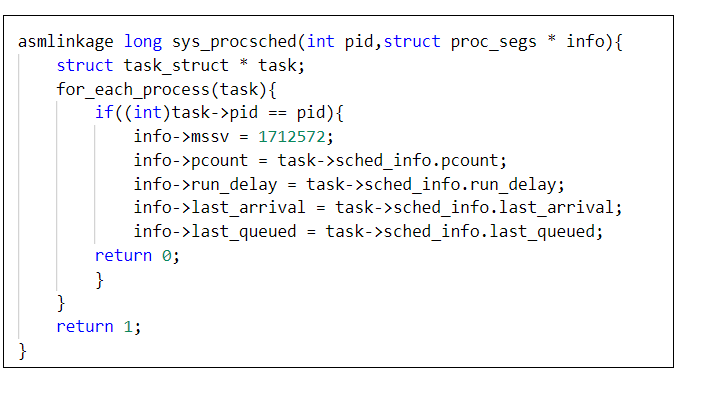
\includegraphics[scale=1.00]{Capture.PNG}
    \end{itemize}
\end{itemize}
\newpage
\section{Compilation and Installation process}
\begin{enumerate}
\item \textbf{Build the configured kernel}
\\
\begin{itemize}
\item Đầu tiên, để build kernel, t chạy lệnh "Make" để tạo file \textit{vmlinuz}. Vì đây là giai đoạn tốn thời gian, ta có thể chạy song song với tag "-j   np" với np là số process ta muốn dùng thực thi công việc.
\item Sau khi biên dịch, \textit{vmlinuz} là một kernel có khả năng khởi động thực tế, "z" để chỉ ra hạt nhân đã được nén.
\item Tiếp đến, tạo modules cho kernel mới, ta dùng lệnh "Make modules", ta cũng có thể sử tag "-j   np" với np là số process ta muốn dùng thực thi công việc để tiết kiệm thời gian.
\end{itemize}
\\
\textbf{QUESTION:} Ý nghĩa của lệnh\textbf{ Make} và \textbf{Make modules }?\\
Make được dùng để build kernel mới, trong khi Make modules để build các
thư viện, mô đun khác.
\item \textbf{Installing the new kernel}
\begin{itemize}
\item Với quyền sudo, ta chạy lệnh "Make modules\_install" để  copy các file kernel modules vào địa chỉ/lib/modules . Lệnh "Make install" để cài đặt kernel mới tạo vào hệ thống.
\item Sau khi đã install, ta thực hiện khởi động lại máy, lúc này, nếu không vì các lý do đặc
biệt, hệ thống của chúng ta sẽ đang sử dụng kernel vừa được install. Vì chúng ta đã
thay đổi số hiệu kernel trong khi thiết lập nên câu lệnh uname -r sẽ cho chúng ta số
hiệu kernel giống vậy. Ở trường hợp này, ta sẽ thấy kết quả là 4.4.56.\textit{MSSV}.
\end{itemize}

\item \textbf{Testing} \\
Sau khi thực hiện xong các hàm, ta viết một test nhỏ sử dụng hàm syscall và kiểm
chứng lại kết quả. Nếu kết quả là MSSV của mình chứng tỏ đã thành công.
\\
     \fbox{
   \parbox{0.8\linewidth}{
       \#include <sys/syscall.h>\\
\#include <stdio.h>\\
\#define SIZE 10\\
 int main() \{\\
 long sysvalue;\\
unsigned long info[SIZE];\\
sysvalue = syscall([number\_32], 1, info);\\
printf({\color{pink}"My MSSV: \%ul\n"}, info[0]);\\
\}
	    }
        }\\
\\
\textbf{QUESTION:} Tại sao chương trình có thể kiểm tra được hệ thống của ta có hoạt động được hay không ?\\
Vì ta dùng syscall() thực hiện gọi gián tiếp vào hệ
thống và lấy một syscall cụ thể từ tham số nhập vào, tham số ở đây là số thứ tự của syscall mà ta vừa thêm vào. Nếu procsched đã thực sự tồn tại trong hệ thống thì nó sẽ được gọi một cách thành công.
\end{enumerate}

\newpage
\section{Making API for system calls}
  
\begin{itemize}
\item Tuy ta đã hiện thực system call sys\_procsched thành công, nhưng việc kích hoạt vẫn khá bất tiện do phải gọi qua số thứ tự. Cho nên đễ đơn giản hơn, ta sẽ tạo một thư viện mới để liên kết động khi có ứng dụng nào đó muốn sử dụng procsched.
\item Tạo file prosched.h ở địa chỉ khác với kernel, và khai báo {\color{blue}struct} proc\_segs một lần nữa, giống với trong file mà được
hiện thực trong kernel.
\\
\\
\textbf{QUESTION:} Tại sao ta lại phải định nghĩa struct trong khi ta đã định nghĩa trước đó ?\\
Ta cần định nghĩa lại struct proc\_segs bởi vì đang viết wrapper ở bên ngoài
thư mục kernel cho nên file procsched.h không có đường dẫn nào đến
struct proc\_segs trong kernel cho nên cần phải định nghĩa lại struct này
để đảm bảo rằng có thể lấy được dữ liệu và gán cho nó.

\item  Tạo file procsched.c để chứa đoạn code cho wrapper, hoàn thành đoạn code tại {\color{blue}\# TODO} như sau : \\
 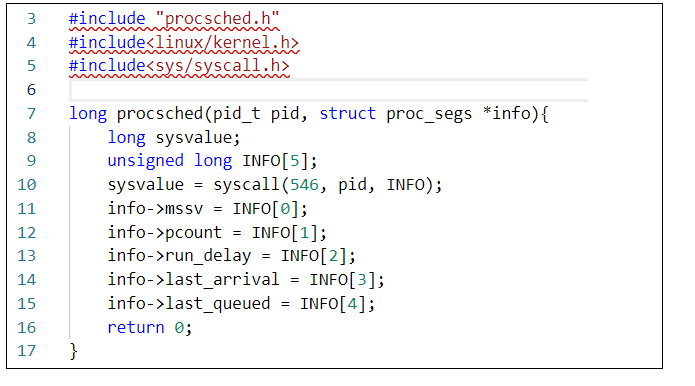
\includegraphics[scale=1.00]{procsched.PNG}
\item Ta đã có file h, nhưng để mọi người có thể sử dụng được (include được), ta cần copy tới
/usr/include, nơi mà biên dịch gcc tìm khi ta dùng lệnh \#include<>:\\
\fbox{
   \parbox{0.8\linewidth}{
		\$ sudo cp <path to procsched.h> /usr/include
	    }
        }
\\
\\
\textbf{QUESTION:} Tại sao ta lại cần root để copy file tới /usr/include?\\
Vì đó là file của hệ thống, người dùng thông thường chỉ có quyền xem không thể sửa đổi. Nên cần root để ta có thể copy file vào /usr.
\item Và để có thể sử dụng trong chương trình khác, ta cần có một object có thể hện thực được:\\
\fbox{
   \parbox{0.8\linewidth}{
		\$ gcc -shared -fpic procsched.c -o libprocsched.so
	    }
        }
\\
\\
\textbf{QUESTION:} Tại sao lại có -shared và -fpic trong câu lệnh ?\\
-shared để tạo các shared object cho các thư viện liên kết. -fpic để đảm bảo trình biên dịch tạo ra code không phụ thuộc địa chỉ. Cả 2 được dùng để tạo thư viện động.
\item Nếu thành công copy file libprocsched.so đến /usr/lib
\item Và cuối cùng, để kiểm tra kết quả, tạo một file mới có sử dụng hàm procsched với pid là id của chính chương trình. Compile với -lprocsched.
\item  So sánh kết quả với /proc/<pid>/maps file. Kêt quả giống nhau là thành công.
\end{itemize}
\section{Conclusion}
\textbf{Bảng phân chia công việc}
\begin{center}
\begin{tabular}{|p{4cm}|p{6cm}|p{3cm} } 
 \hline
 Thành viên  & Công việc & Tỉ lệ đóng góp\\ \hline
 Nguyễn Tiến Phát & Hiện thực sys\_procsched, build kernel, viết báo cáo & 50\%\\\hline 
 Nguyễn Lục Sâm Bảo & hiện thực wrapper, build kernel, viết báo cáo & 50\%\\
 \hline
\end{tabular}
\end{center}
\textbf{Reference}
\begin{enumerate}
\item \textit{Linux Kernel In A Nutshell} by Greg Kroah-Hartman
\item \textit{Adding a Syscall to Linux 3.14} - Shane Tully
\item \textit{https://kernelnewbies.org/KernelBuild}
\end{enumerate}

\end{document}